% !TeX root = RJwrapper.tex
\title{ggplot2 Compatible Quantile-Quantile Plots in R}
\author{by Alexandre Almeida, Adam Loy, Heike Hofmann}

\maketitle

\abstract{%
Q-Q plots allow us to assess univariate distributional assumptions by
comparing a set of quantiles from the empirical and the theoretical
distributions in the form of a scatterplot. To aid in the interpretation
of Q-Q plots, reference lines and confidence bands are often added. We
can also detrend the Q-Q plot so the vertical comparisons of interest
come into focus. Various implementations of Q-Q plots exist in R, but
none implements all of these features. \pkg{qqplotr} extends
\pkg{ggplot2} to provide a complete implementation of Q-Q plots. This
paper introduces the plotting framework provided by \pkg{qqplotr} and
provides multiple examples of how it can be used.
}

\newcommand{\hh}[1]{{\textcolor{orange}{#1}}}
\newcommand{\al}[1]{{\textcolor{violet}{#1}}}
\newcommand{\Aa}[1]{{\textcolor{olive}{#1}}}

\subsection{Background}\label{background}

\label{sec:background}

Univariate distributional assessment is a common thread throughout
statistical analyses during both the exploratory and confirmatory
stages. When we begin exploring a new data set we often consider the
distribution of individual variables before moving on to explore
multivariate relationships. After a model has been fit to a data set, we
must assess whether the distributional assumptions made are reasonable,
and if they are not, then we must understand the impact this has on the
conclusions of the model. Graphics provide arguably the most common way
to carry out these univariate assessments. While there are many plots
that can be used for distributional exploration and assessment, a
quantile-quantile (Q-Q) plot \citep{Wilk1968-ii} is one of the most
common plots used.

Q-Q plots compare two distributions by matching a common set of
quantiles. To compare a sample, \(y_1, y_2, \ldots, y_n\), to a
theoretical distribution, a Q-Q plot is simply a scatterplot of the
sample quantiles, \(y_{(i)}\), against the corresponding quantiles from
the theoretical distribution, \(F^{-1}\left( F_n(y_{(i)}) \right)\). If
the empirical distribution is consistent with the theoretical
distribution, then the points will fall on a line. For example, Figure
\ref{fig:ex-qq1} shows two Q-Q plots: the left plot compares a sample
drawn from a lognormal distribution to a lognormal distribution, while
the right plot compares a sample drawn from a lognormal distribution to
a normal distribution. As expected, the lognormal Q-Q plot is
approximately linear, as the data and model are in agreement, while the
normal Q-Q plot is curved, indicating disagreement between the data and
the model.

\begin{Schunk}
\begin{figure}

{\centering 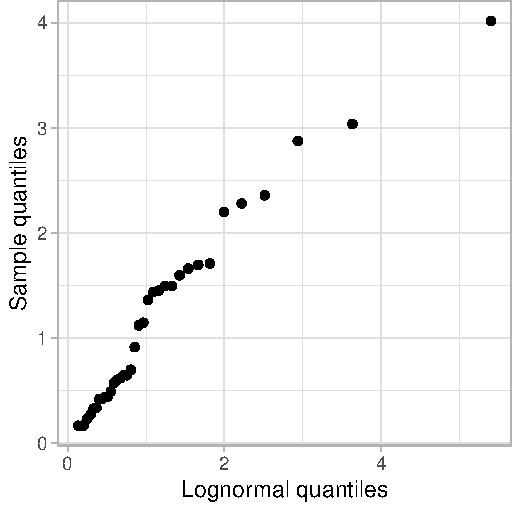
\includegraphics[width=0.4\linewidth]{loy-figures/ex-qq1-1} 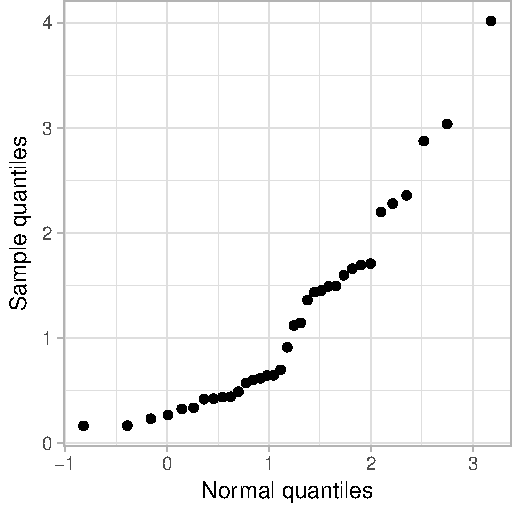
\includegraphics[width=0.4\linewidth]{loy-figures/ex-qq1-2} 

}

\caption[The left plot compares a sample drawn from a lognormal distribution to a lognormal distribution, while the right plot compares a sample drawn from a lognormal distribution to a normal distribution]{The left plot compares a sample drawn from a lognormal distribution to a lognormal distribution, while the right plot compares a sample drawn from a lognormal distribution to a normal distribution. The curvature in the normal Q-Q plot highlights the disagreement betweeen the data and the model.}\label{fig:ex-qq1}
\end{figure}
\end{Schunk}

Additional graphical elements are often added to Q-Q plots in order to
aid in distributional assessment. A reference line is often added to a
Q-Q plot to help detection of departures from the proposed model. This
line is often drawn either by tracing the identity line or by connecting
two pairs of quantiles, such as the first and third quartiles, which is
known as the Q-Q line. Pointwise or simultaneous confidence bands are
also frequently built around the reference line to display the expected
degree of sampling error for the proposed model. Such bands help gauge
how troubling a departure from the proposed model may be. Figure
\ref{fig:ex-qq2} adds Q-Q lines and 95\% pointwise confidence bands to
the Q-Q plots in Figure \ref{fig:ex-qq1}.

\begin{Schunk}
\begin{figure}

{\centering 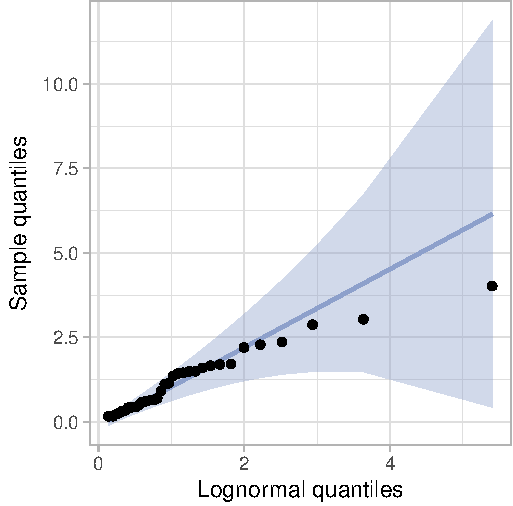
\includegraphics[width=.4\linewidth]{loy-figures/ex-qq2-1} 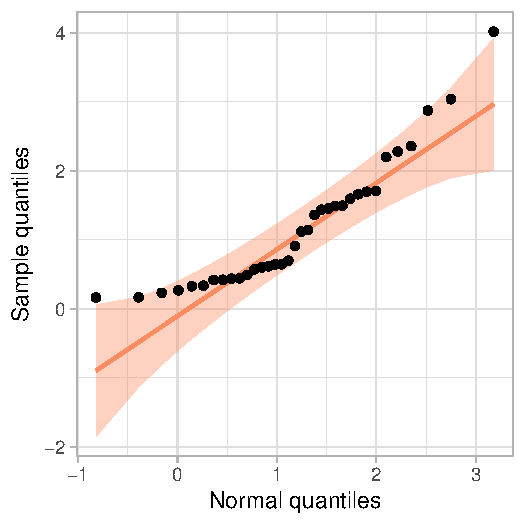
\includegraphics[width=.4\linewidth]{loy-figures/ex-qq2-2} 

}

\caption[Adding reference lines and $95\%$ pointwise confidence bands to the Q-Q plots in Figure 1]{Adding reference lines and $95\%$ pointwise confidence bands to the Q-Q plots in Figure 1.}\label{fig:ex-qq2}
\end{figure}
\end{Schunk}

Different orientations of Q-Q plots have also been proposed, most
notably the detrended Q-Q plot. To detrend a Q-Q plot, the \(y\)-axis is
changed to show the difference between the observed quantile and the
reference line. Consequently, the \(x\)-axis represents agreement with
the theoretical distribution. \citet{Loy2016-fg} find that detrended Q-Q
plots are more powerful than other designs, as long as the \(x\)- and
\(y\)-axes are adjusted to ensure that distances in the \(x\)- and
\(y\)-directions are on the same scale. This Q-Q plot design is called
an \emph{adjusted detrended Q-Q plot}. Without this adjustment to the
range of the axes, \emph{ordinary detrended Q-Q plots} are produced,
which were found to have lower power than the standard Q-Q plot in some
situations \citep{Loy2016-fg}, while the adjusted detrended Q-Q plots
were found to be consistently more powerful. Figure \ref{fig:ex-detrend}
displays the normal Q-Q plot from Figure \ref{fig:ex-qq2} along with its
adjusted detrended version.

\begin{Schunk}
\begin{figure}

{\centering 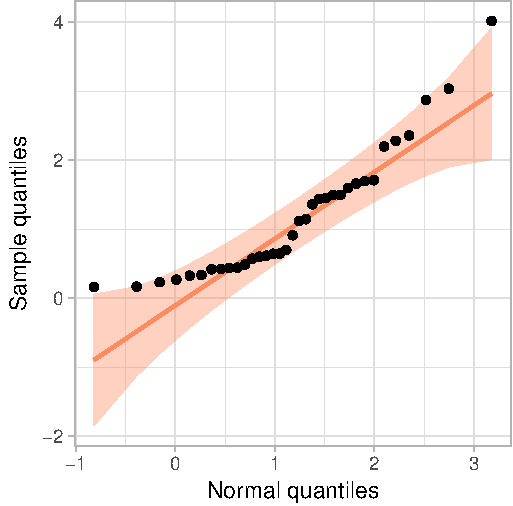
\includegraphics[width=.4\linewidth]{loy-figures/ex-detrend-1} 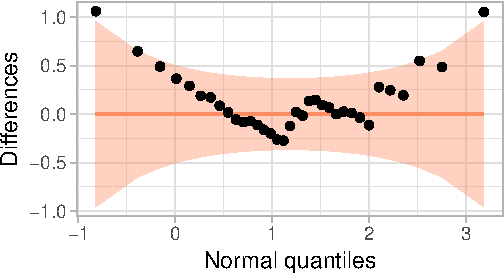
\includegraphics[width=.4\linewidth]{loy-figures/ex-detrend-2} 

}

\caption[The left plot displays a traditional normal Q-Q plot for data simulated from a lognormal distribution]{The left plot displays a traditional normal Q-Q plot for data simulated from a lognormal distribution. The right plot displays an adjusted detrended Q-Q plot of the same data, created by plotting the differences between the sample quantiles and the proposed model on the $y$-axis.}\label{fig:ex-detrend}
\end{figure}
\end{Schunk}

Various implementations of Q-Q plots exist in R. Normal Q-Q plots, where
a sample is compared to the Standard Normal Distribution, are
implemented using \texttt{qqnorm} and \texttt{qqline} in \pkg{base}
graphics \citep{R}. \texttt{qqplot} provides a more general approach in
base R that allows a specification of a second vector of quantiles,
enabling comparisons to distributions other than a Normal. Similarly,
the \pkg{lattice} package provides a general framework for Q-Q plots in
the \texttt{qqmath} function, allowing the analyst to compare a sample
to any theoretical distribution by specifying the appropriate quantile
function \citep{lattice}. \texttt{qqPlot} in the \pkg{car} package also
allows for the assessment of non-normal distributions and adds pointwise
confidence bands via normal theory or the parametric bootstrap
\citep{car}. The \pkg{ggplot2} package provides \texttt{geom\_qq} and
\texttt{geom\_qq\_line}, enabling the creation of Q-Q plots with a
reference line, much like those created using \texttt{qqmath}
\citep{ggplot2}. None of these general-use packages allow for easy
construction of detrended Q-Q plots.

The \pkg{qqplotr} package extends \pkg{ggplot2} to provide a complete
implementation of Q-Q plots. The package allows for quick construction
of all Q-Q plot designs without sacrificing the flexibility of the
\pkg{ggplot2} framework. In the remainder of this paper, we introduce
the plotting framework provided by \pkg{qqplotr} and provide multiple
examples of how it can be used.

\subsection{\texorpdfstring{Implementing Q-Q plots in the \pkg{ggplot2}
framework}{Implementing Q-Q plots in the  framework}}\label{implementing-q-q-plots-in-the-framework}

\label{sec:implementing}

\pkg{qqplotr} provides a \pkg{ggplot2} layering mechanism for Q-Q
points, reference lines, and confidence bands by implementing separate
statistical transformations (\texttt{stat}s). In this section, we
describe each transformation.

\subsubsection{\texorpdfstring{\texttt{stat\_qq\_point}}{stat\_qq\_point}}\label{stat_qq_point}

This modified version of \texttt{stat\_qq}/\texttt{geom\_qq} (from
\pkg{ggplot2}) plots the sample quantiles against the theoretical
quantiles, as shown in Figure \ref{fig:ex-qq1}. The novelty of this
implementation is an option to detrend the plotted points. All other
transformations in \pkg{qqplotr} also allow for the detrend option.
Below we present a complete call to \texttt{stat\_qq\_point} and
highlight the default values of its parameters:

\begin{Schunk}
\begin{Sinput}
stat_qq_point(data = NULL,
              mapping = NULL,
              geom = "point",
              position = "identity",
              na.rm = TRUE,
              show.legend = NA,
              inherit.aes = TRUE,
              distribution = "norm",
              dparams = list(),
              detrend = FALSE,
              identity = FALSE,
              qtype = 7,
              qprobs = c(0.25, 0.75),
              ...)
\end{Sinput}
\end{Schunk}

\begin{itemize}
\item
  Parameters such as \texttt{data}, \texttt{mapping}, \texttt{geom},
  \texttt{position}, \texttt{na.rm}, \texttt{show.legend}, and
  \texttt{inherit.aes} are commonly found among several \pkg{ggplot2}
  transformations.
\item
  \texttt{distribution} is a character string that sets the theoretical
  probability distribution. Here, we followed the nomenclature from the
  \pkg{stats} package, but rather than requiring the full function name
  for a distribution (e.g., \texttt{"dnorm"}), only the suffix is
  required (e.g., \texttt{"norm"}). If you wish to provide a custom
  distribution, then you must first create its density (PDF),
  distribution (CDF), quantile, and simulation functions, following the
  nomenclature outlined in \pkg{stats}. For example, to create the
  \texttt{"custom"} distribution, you must provide the appropriate
  \texttt{dcustom}, \texttt{pcustom}, \texttt{qcustom}, and
  \texttt{rcustom} functions. A detailed example is given in the
  \nameref{sec:user-dists} section.
\item
  \texttt{dparams} is a named list specifying the parameters of the
  proposed \texttt{distribution}. By default, maximum likelihood
  etimates (MLEs) are used, so specifying this argument overrides the
  MLEs. Please note that MLEs are currently only supported for
  distributions available in \pkg{stats}, so if a custom distribution is
  provided to \texttt{distribution}, then \emph{all} of its parameters
  must be estimated and passed as a named list to \texttt{dparams}.
\item
  \texttt{detrend} is a logical that controls whether the points should
  be detrended (as shown in Figure \ref{fig:ex-detrend}), producing
  ordinary detrended Q-Q plots. For additional details on how to use
  this parameter and produce the more powerful adjusted detrended Q-Q
  plots, see the \nameref{sec:detrending} section.
\item
  \texttt{identity} is a logical value used in the case of detrending,
  i.e.~\texttt{detrend\ =\ TRUE}. If \texttt{identity\ =\ FALSE}
  (default), then the points will be detrended according to the
  traditional Q-Q line that intersects the two data quantiles specified
  by \code{qprobs} (see below). If \texttt{identity\ =\ TRUE}, the
  identity line will be used instead as the reference line when
  constructing the detrended Q-Q plot.
\item
  \texttt{qtype} and \texttt{qprobs} are only used when
  \texttt{detrend\ =\ TRUE} \emph{and} \texttt{identity\ =\ FALSE}.
  These parameters are passed to the \texttt{type} and \texttt{probs}
  parameters of the \texttt{quantile} function from \pkg{stats}, both of
  which are used to specify which quantiles are used to form the Q-Q
  line.
\end{itemize}

\subsubsection{\texorpdfstring{\texttt{stat\_qq\_line}}{stat\_qq\_line}}\label{stat_qq_line}

The \texttt{stat\_qq\_line} statistical transformation draws a reference
line in a Q-Q plot.

\begin{Schunk}
\begin{Sinput}
stat_qq_line(data = NULL,
             mapping = NULL,
             geom = "path",
             position = "identity",
             na.rm = TRUE,
             show.legend = NA,
             inherit.aes = TRUE,
             distribution = "norm",
             dparams = list(),
             detrend = FALSE,
             identity = FALSE,
             qtype = 7,
             qprobs = c(0.25, 0.75),
             ...)
\end{Sinput}
\end{Schunk}

Nearly all of the parameters for \texttt{stat\_qq\_line} are identical
to those for \texttt{stat\_qq\_point}. Hence, with the exception of
\texttt{identity}, all other parameters have the same interpretation.
For \texttt{stat\_qq\_line}, the \texttt{identity} parameter is
\emph{always} used, regardless of the value of \texttt{detrend}. This
parameter controls which reference line is drawn:

\begin{enumerate}
\def\labelenumi{\alph{enumi})}
\tightlist
\item
  When \texttt{identity\ =\ FALSE} (default), the \emph{Q-Q line} is
  drawn. By default the Q-Q line is drawn through two points, the .25
  and .75 quantiles of the theoretical and empirical distributions. This
  line provides a robust estimate of the empirical distribution, which
  is of particular advantage for small samples \citep{Loy2016-fg}.
\item
  When \texttt{identity\ =\ TRUE}, the \emph{identity line} is drawn. By
  definition of a Q-Q plot the \emph{identity line} represents the
  theoretical distribution.
\end{enumerate}

Both of these reference lines have a special meaning in the context of
Q-Q plots. By comparing these two lines we learn about how well the
parameters estimated from the sample match the theoretical parameters.
For a distributional family that is invariant to linear transformations,
the parameters specified in the theoretical distribution only have an
effect on the Q-Q line and the Q-Q points---that is, the parameters get
shifted and scaled in the plot, but relative relationships do not change
aside from a change of scale on the \(x\)-axis. For other distributions,
such as a lognormal distribution, re-specifications of the parameters
result in non-linear transformations of the Q-Q line and Q-Q points (see
Figure \ref{fig:qqline} for an example).

\begin{Schunk}
\begin{figure}

{\centering 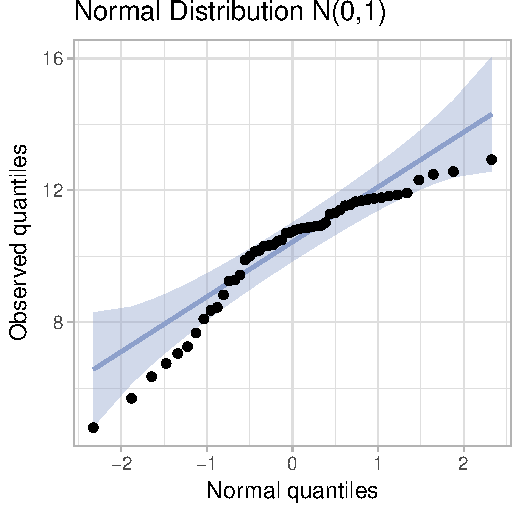
\includegraphics[width=0.4\linewidth]{loy-figures/qqline-1} 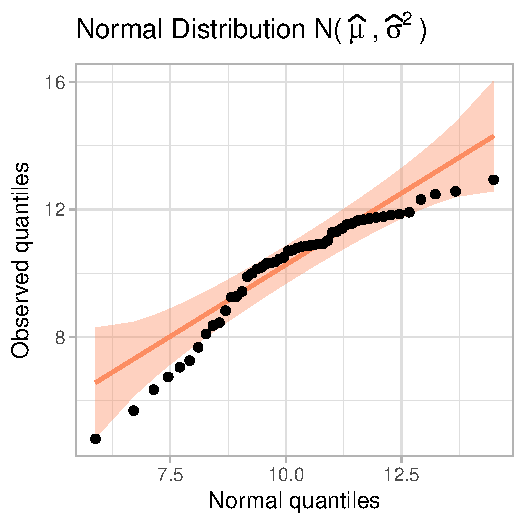
\includegraphics[width=0.4\linewidth]{loy-figures/qqline-2} 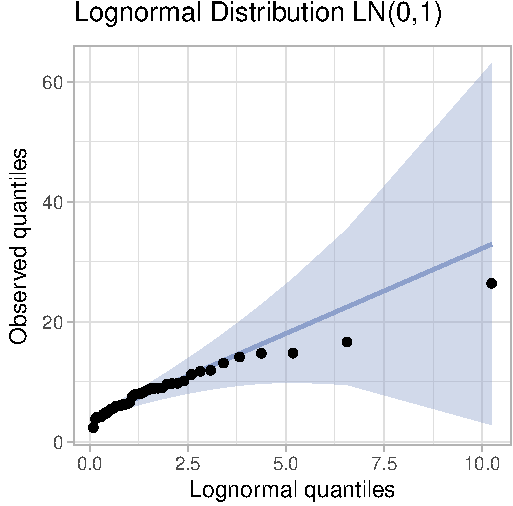
\includegraphics[width=0.4\linewidth]{loy-figures/qqline-3} 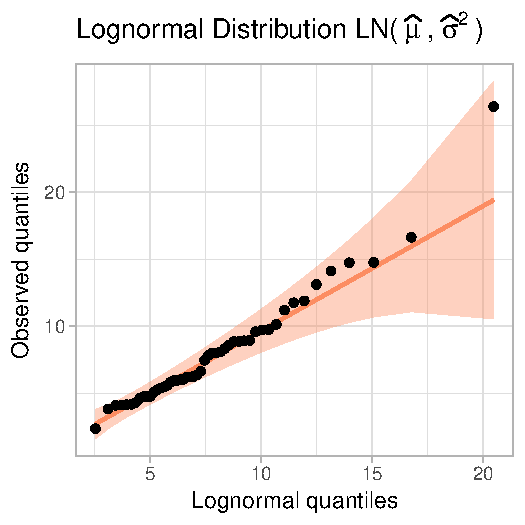
\includegraphics[width=0.4\linewidth]{loy-figures/qqline-4} 

}

\caption[Q-Q plots of (top-left) a Standard Normal distribution, (top-right) a normal distribution with ML parameter estimates]{Q-Q plots of (top-left) a Standard Normal distribution, (top-right) a normal distribution with ML parameter estimates. Only the scales on the axes change between these plots. The bottom two plots show Q-Q plots of the same sample from a lognormal distribution. On the left, the mean and variance are 0 and 1, respectively, on the log scale. On the right, ML estimates for mean and variance are used.}\label{fig:qqline}
\end{figure}
\end{Schunk}

\subsubsection{\texorpdfstring{\texttt{stat\_qq\_band}}{stat\_qq\_band}}\label{stat_qq_band}

Confidence bands can be drawn around the reference line using one of
three methods: a pointwise normal approximation, the parametric
bootstrap, or the tail-sensitive procedure \citep{Aldor-Noiman2013-xw}.

\begin{Schunk}
\begin{Sinput}
stat_qq_band(data = NULL,
             mapping = NULL,
             geom = "qq_band",
             position = "identity",
             show.legend = NA,
             inherit.aes = TRUE,
             na.rm = TRUE,
             distribution = "norm",
             dparams = list(),
             detrend = FALSE,
             identity = FALSE,
             qtype = 7,
             qprobs = c(0.25, 0.75),
             bandType = "normal",
             B = 1000,
             conf = 0.95,
             mu = NULL,
             sigma = NULL,
             ...)
\end{Sinput}
\end{Schunk}

\begin{itemize}
\item
  \texttt{bandType} is a character string controlling the method used to
  construct the confidence bands:

  \begin{itemize}
  \tightlist
  \item
    \textbf{Normal:} Specifying \texttt{bandType\ =\ "normal"}
    constructs pointwise confidence bands based on a normal
    approximation to the distribution of the order statistics. For
    example, an approximate 95\% confidence interval for the \(i\)th
    order statistic is
    \(\widehat{X}_{(i)}~\pm~\Phi^{-1}(.975)~\cdot~SE(X_{(i)})\), where
    \(\widehat{X}_{(i)}\) denotes the value along the fitted reference
    line, \(\Phi^{-1}(\cdot)\) denotes the quantile function for the
    Standard Normal Distribution, and \(SE(X_{(i)})\) is the standard
    error of the \(i\)th order statistic.
  \item
    \textbf{Bootstrap:} Specifying \texttt{bandType\ =\ "boot"}
    constructs pointwise confidence bands using percentile confidence
    intervals from the parametric bootstrap.
  \item
    \textbf{Tail-sensitive:} Specifying \texttt{bandType\ =\ "ts"}
    constructs the simulation-based tail-sensitive simultaneous
    confidence bands proposed by \citet{Aldor-Noiman2013-xw}. Currently,
    tail-sensitive bands are \emph{only} implemented for
    \texttt{distribution\ =\ "norm"}.
  \end{itemize}
\item
  \texttt{B} is a dual-purpose integer parameter---if
  \texttt{bandType\ =\ "boot"}, it specifies the number of bootstrap
  replicates, if \texttt{bandType\ =\ "ts"}, it specifies the number of
  simulated samples necessary to construct the tail-sensitive bands.
\item
  \texttt{conf} is a numerical variable bound between 0 and 1 that sets
  the confidence level of the bands.
\item
  \texttt{mu} and \texttt{sigma} are only used when
  \texttt{bandType\ =\ "ts"}. They represent the center and scale
  parameters, respectively, used to construct the simulated
  tail-sensitive confidence bands. If either is \texttt{NULL}, then
  \emph{both} of the parameters are estimated using robust estimates via
  the \pkg{robustbase} package \citep{robustbase}. Currently,
  \texttt{bandType\ =\ "ts"} is only implemented for
  \texttt{distribution\ =\ "norm"}, which is the only distribution
  discussed by \citet{Aldor-Noiman2013-xw}.
\end{itemize}

\subsubsection{\texorpdfstring{Groups in
\texttt{qqplotr}}{Groups in qqplotr}}\label{groups-in-qqplotr}

\texttt{qqplotr} is implemented in accordance with the \pkg{ggplot2}
concept of groups. When the user maps values to aesthetics that
explicitly (by using \texttt{group}) or implicitly (such as
\texttt{shape} or discrete values of \texttt{colour}, \texttt{size},
etc.) introduce groups, the corresponding calculations respect the
grouping in the data. All groups are compared to the same distributional
family, but the parameters are estimated \emph{separately} for each of
the groups if \texttt{dparams} is not specified (which is the default
for all transformations). If the user wants to fit the \emph{same}
distribution (i.e., the same parameter estimates) to each group, then
the estimates must be manually calculated and passed to \texttt{dparams}
as a named list for each of the desired \pkg{qqplotr} transformations.
The use of groups is illustrated in more detail in the
\nameref{sec:brfss} section.

\FloatBarrier

\subsection{Examples}\label{examples}

\label{sec:examples}

In this section, we demonstrate the capabilities of \pkg{qqplotr} by
providing multiple examples of how the package can be used. We start by
loading the package:

\begin{Schunk}
\begin{Sinput}
library(qqplotr)
\end{Sinput}
\end{Schunk}

\subsubsection{\texorpdfstring{Constructing Q-Q plots with
\texttt{qqplotr}}{Constructing Q-Q plots with qqplotr}}\label{constructing-q-q-plots-with-qqplotr}

To give a brief introduction on how to use \pkg{qqplotr} and its
transformations, consider the \texttt{urine} dataset from the \pkg{boot}
package. This small dataset consists of 79 urine specimens that were
analyzed to determine if certain physical characteristics of the urine
(e.g., pH or urea concentration) might be related to the formation of
calcium oxalate crystals. In this example, we focus on the
distributional assessment of pH measurements made on the samples.

We start by creating a normal Q-Q plot of the data. The top-left plot in
Figure \ref{fig:urine-qq-bands} shows a Q-Q plot comparing the pH
measurements to the normal distribution. The code used to create this
plot is shown below. As previously noted, the parameters of the normal
distribution are automatically estimated using the MLEs, when the
parameters are not specified otherwise in \texttt{dparams}. The shaded
region represents the area between the normal pointwise confidence
bands. As we can see, the distribution of urine pH measurements is
somewhat right-skewed.

\begin{Schunk}
\begin{Sinput}
data(urine, package = "boot")
urine %>% 
  ggplot(aes(sample = ph)) + 
  stat_qq_band(bandType = "normal", fill = "#8DA0CB", alpha = 0.4) + 
  stat_qq_line(colour = "#8DA0CB") +
  stat_qq_point() +
  ggtitle("Normal") +
  xlab("Normal quantiles") +
  ylab("pH measurements quantiles") +
  theme_light() +
  ylim(3.2, 8.7)
\end{Sinput}
\end{Schunk}

Figure \ref{fig:urine-qq-bands} provides an overview of \pkg{qqplotr}'s
capabilities:

\begin{itemize}
\item
  The left column displays Q-Q plots with 95\% pointwise confidence
  bands obtained from a normal approximation.
\item
  The center column displays Q-Q plots with 95\% pointwise confidence
  bands constructed using a parametric bootstrap.
\item
  The right column displays Q-Q plots with 95\% tail-sensitive
  confidence bands.
\item
  The bottom row shows the detrended versions of the Q-Q plots in the
  top row.
\end{itemize}

\begin{Schunk}
\begin{figure}

{\centering 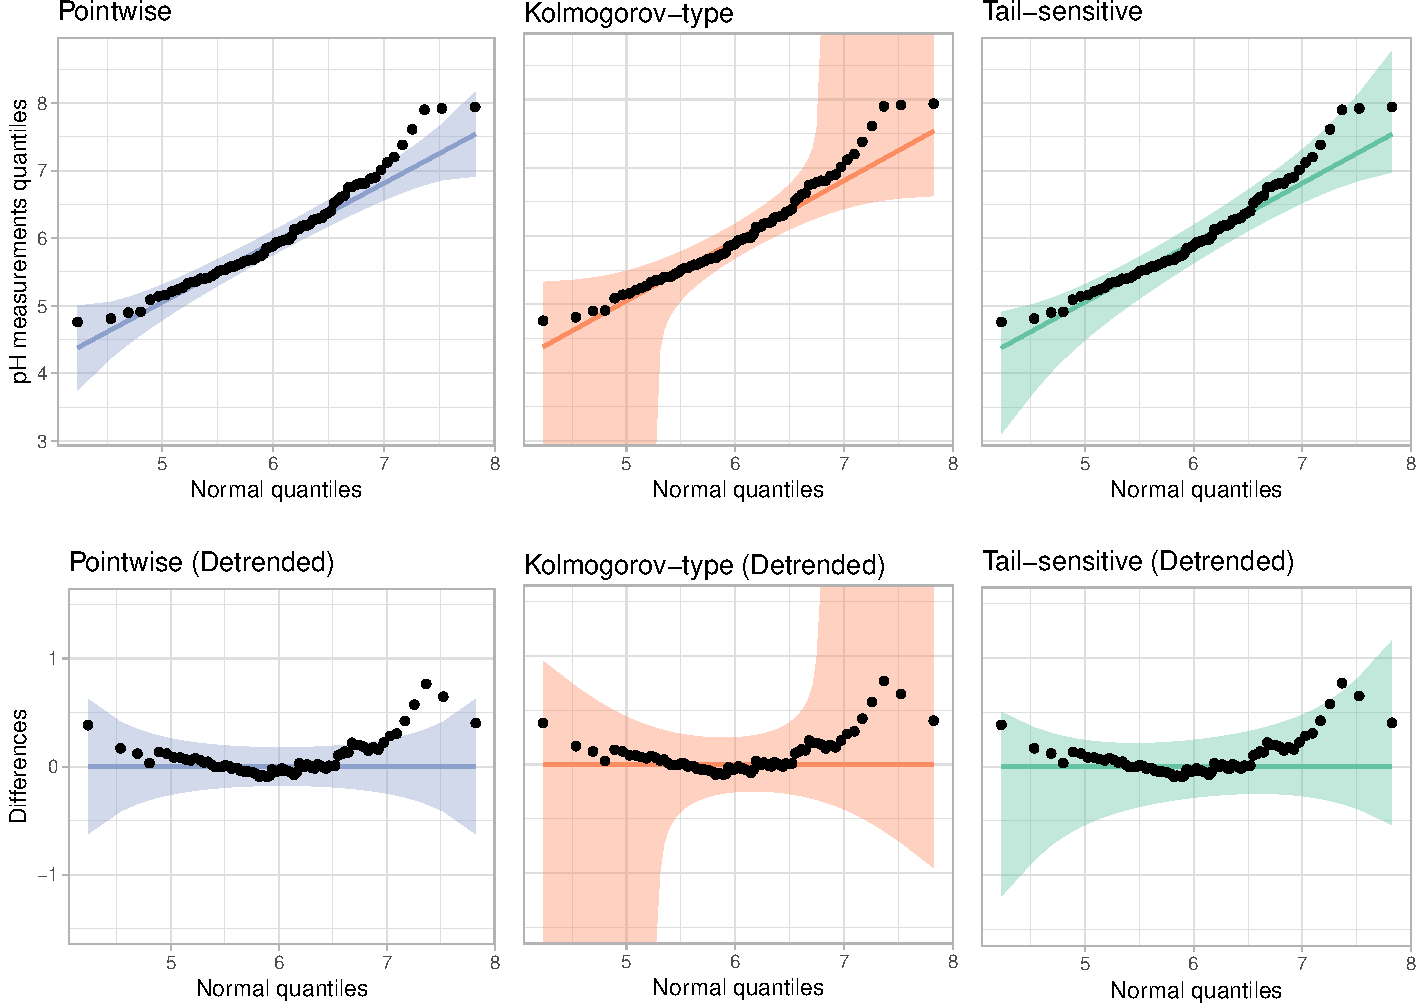
\includegraphics[width=\textwidth]{loy-figures/urine-qq-bands-1} 

}

\caption[Normal Q-Q plots of pH measurements from urine samples using different confidence bands]{Normal Q-Q plots of pH measurements from urine samples using different confidence bands. Depending on the type of confidence band used, we come to different conclusions.}\label{fig:urine-qq-bands}
\end{figure}
\end{Schunk}

\FloatBarrier

\subsubsection{User-provided
distributions}\label{user-provided-distributions}

\label{sec:user-dists}

Using the capabilities of \pkg{qqplotr} with the distributions
implemented in \pkg{stats} is relatively straightfoward, since the
implementation allows you to specify the suffix (i.e., distribution and
or abbreviation) via the \texttt{distribution} argument and the
parameter estimates via the \texttt{dparams} argument. However, there
are times when the distributions in \pkg{stats} are not sufficient for
the demands of the analysis. For example, there is no left-skewed
distribution listed aside from the Beta Distribution, which has a
restrictive support. User-coded distributions, or distributions from
other packages, can be used with \pkg{qqplotr} as long as the
distributions are defined following the conventions laid out in
\pkg{stats}. Specfically, for some distribution there must be
density/mass (\texttt{d} prefix), CDF (\texttt{p} prefix), quantile
(\texttt{q} prefix), and simulation (\texttt{r} prefix) functions. In
this section, we illustrate the use of the smallest extreme value
distribution (SEV).

To qualify for the 2012 Olympics in the men's long jump, athletes had to
meet/exceed the 8.1 meter standard or place in the top twelve. During
the qualification events, each athlete was able to jump up to three
times, using their best (i.e., longest) jump as the result. Figure
\ref{fig:jump-density} shows a density plot of the results, which is
clearly left skewed.

We start by loading the \texttt{longjump} dataset included in
\pkg{qqplotr} and removing any \texttt{NA}s:

\begin{Schunk}
\begin{Sinput}
data("longjump", package = "qqplotr")
longjump <- na.omit(longjump)
\end{Sinput}
\end{Schunk}

\begin{Schunk}
\begin{figure}

{\centering 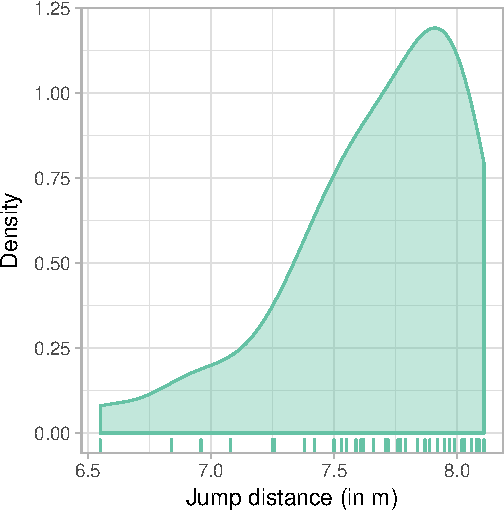
\includegraphics[width=0.45\linewidth]{loy-figures/jump-density-1} 

}

\caption[Density and rug plot of the 2012 men's long jump qualifying round]{Density and rug plot of the 2012 men's long jump qualifying round. The distances are clearly left skewed.}\label{fig:jump-density}
\end{figure}
\end{Schunk}

Next, we define the suite of distributional functions necessary to
utilize the SEV distribution.

\begin{Schunk}
\begin{Sinput}
# CDF
psev <- function(q, mu = 0, sigma = 1) {
  z <- (q - mu) / sigma
  1 - exp(-exp(z))
}

# PDF
dsev <- function(x, mu = 0, sigma = 1) {
  z <- (x - mu) / sigma
  (1 / sigma) * exp(z - exp(z))
}

# Quantile function
qsev <- function(p, mu = 0, sigma = 1) {
  mu + log(-log(1 - p)) * sigma
}

# Simulation function
rsev <- function(n, mu = 0, sigma = 1) {
  qsev(runif(n), mu, sigma)
}
\end{Sinput}
\end{Schunk}

With the \texttt{*sev} distribution functions in hand, we can create a
Q-Q plot to assess the appropriateness of the SEV model (Figure
\ref{fig:sev-qq}). The Q-Q plot shows that the distances do not
substantially deviate from the SEV model, so we have found an adequate
representation of the distances. The code used to create Figure
\ref{fig:sev-qq} is given below:

\begin{Schunk}
\begin{Sinput}
ggplot(longjump, aes(sample = distance)) +
  stat_qq_band(distribution = "sev", 
               dparams = list(mu = 0, sigma = 1),
               fill = "#8DA0CB",
               alpha = 0.4) +
  stat_qq_line(distribution = "sev", 
               colour = "#8DA0CB",
               dparams = list(mu = 0, sigma = 1)) +
  stat_qq_point(distribution = "sev", 
                dparams = list(mu = 0, sigma = 1)) +
  xlab("SEV quantiles") +
  ylab("Jump distance (in m)") +
  theme_light()
\end{Sinput}
\begin{figure}

{\centering 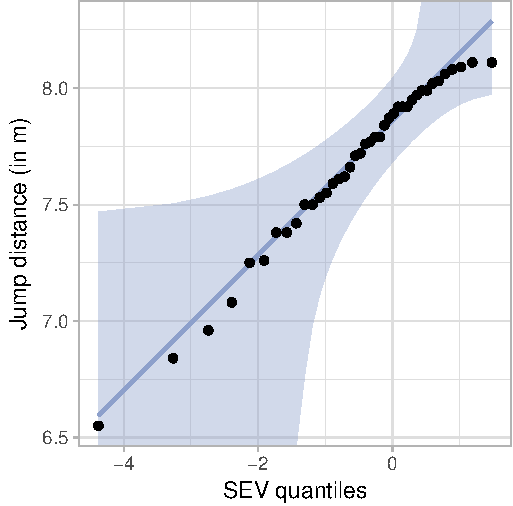
\includegraphics[width=0.45\linewidth]{loy-figures/sev-qq-1} 

}

\caption[Q-Q plot comparing the long jump distances to the standard SEV distribution with 95\% pointwise confidence bands]{Q-Q plot comparing the long jump distances to the standard SEV distribution with 95\% pointwise confidence bands. The SEV distribution appears to adequately model the distances.}\label{fig:sev-qq}
\end{figure}
\end{Schunk}

\FloatBarrier

\subsubsection{Detrending Q-Q plots}\label{detrending-q-q-plots}

\label{sec:detrending}

To illustrate how to construct an adjusted detrended Q-Q plot using
\pkg{qqplotr}, consider detrending Figure \ref{fig:sev-qq}. This is done
by adding the argument \texttt{detrend\ =\ TRUE} to
\texttt{stat\_qq\_point}, \texttt{stat\_qq\_line}, and
\texttt{stat\_qq\_band}. To adjust the aspect ratio to ensure that
vertical and horizontal distances are on the same scale we further add
\texttt{coord\_fixed(ratio\ =\ 1)}. We leave it to the user to adjust
the \(y\)-axis limits on a case-by-case basis. The full command to
construct Figure \ref{fig:detrend-sev} is given below:

\begin{Schunk}
\begin{Sinput}
ggplot(longjump, aes(sample = distance)) +
  stat_qq_band(distribution = "sev",
               detrend = TRUE,
               dparams = list(mu = 0, sigma = 1),
               fill = "#8DA0CB",
               alpha = 0.4) +
  stat_qq_line(distribution = "sev",
               detrend = TRUE,
               dparams = list(mu = 0, sigma = 1),
               colour = "#8DA0CB") +
  stat_qq_point(distribution = "sev",
                detrend = TRUE,
                dparams = list(mu = 0, sigma = 1)) +
  xlab("SEV quantiles") +
  ylab("Differences") +
  theme_light() + 
  coord_fixed(ratio = 1, ylim = c(-2, 2))
\end{Sinput}
\begin{figure}

{\centering 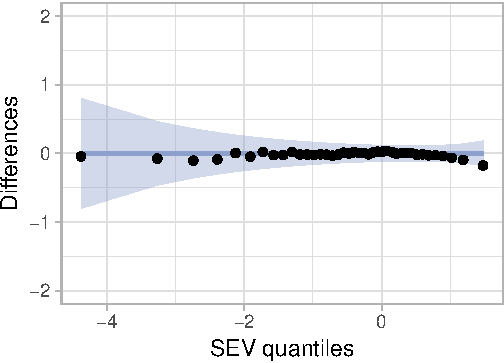
\includegraphics[width=0.45\linewidth]{loy-figures/detrend-sev-1} 

}

\caption[An adjusted detrended Q-Q plot assessing the appropriateness of the SEV distribution for the long jump data]{An adjusted detrended Q-Q plot assessing the appropriateness of the SEV distribution for the long jump data.}\label{fig:detrend-sev}
\end{figure}
\end{Schunk}

\subsubsection{BRFSS example}\label{brfss-example}

\label{sec:brfss}

The Center for Disease Control and Prevention runs an annual telephone
survey, the Behavioral Risk Factor Surveillance System (BRFSS), to keep
track of the US populations' ``health-related risk behaviors, chronic
health conditions, and use of preventive services'' \citep{brfss}. Close
to half a million interviews are conducted each year. In this example,
we focus on the responses for Iowa in 2012. The data set consists of
7166 responses across 359 questions and derived variables. To further
illustrate the functionality of \pkg{qqplotr}, we focus on assessing the
distributions of Iowan's heights and weights.

Figure \ref{fig:heights} shows two Q-Q plots constructed from a sample
of 200 men and 200 women drawn from the overall number of responses. On
the left-hand side, individuals' heights are displayed in a Q-Q plot
comparing raw heights to a normal distribution. We see that the
distributions for both men and women (colour) show horizontal steps:
this indicates that the distributional assessement is heavily dominated
by the discreteness in the data, as most respondents provided their
height to the nearest inch. On the right-hand side of Figure
\ref{fig:heights}, we use jittering to remedy this situation---that is,
we add a random number generated from a random uniform distribution on
\(\pm 0.5\) inch to the reported height, as shown in the code below:

\begin{Schunk}
\begin{Sinput}
data("iowa", package = "qqplotr")
set.seed(3145)

sample_ia <- iowa %>% 
  tidyr::nest(-SEX) %>% 
  mutate(
    data = data %>% 
    purrr::map(.f = function(x) sample_n(x, size = 200))
    ) %>% 
  tidyr::unnest(data) %>% 
  dplyr::select(SEX, WTKG3, HTIN4) %>%
  mutate(Gender = c("Male", "Female")[SEX])

params <- iowa %>% 
  filter(!is.na(HTIN4)) %>% 
  summarize(m = mean(HTIN4), s = sd(HTIN4))

customization <- list(scale_fill_brewer(palette = "Set2"),
                      scale_colour_brewer(palette = "Set2"),
                      xlab("Normal quantiles"),
                      ylab("Height (in.)"),
                      coord_equal(),
                      theme_light(),
                      theme(legend.position = c(0.8, 0.2), aspect.ratio = 1))

sample_ia %>% 
  ggplot(aes(sample = HTIN4, colour=Gender, fill=Gender)) + 
  stat_qq_band(alpha = 0.4,
               dparams = list(mean = params$m, sd = params$s)) + 
  stat_qq_line(dparams = list(mean = params$m, sd = params$s)) + 
  stat_qq_point(dparams = list(mean = params$m, sd = params$s)) +
  customization

sample_ia %>% 
  mutate(HTIN4.jitter = jitter(HTIN4, factor = 2)) %>% 
  ggplot(aes(sample = HTIN4.jitter, colour = Gender, fill = Gender)) + 
  geom_abline(slope = 1, intercept = 0, colour = "grey40") +
  stat_qq_band(alpha = 0.4,
               dparams = list(mean = params$m, sd = params$s)) +
  stat_qq_line(dparams = list(mean = params$m, sd = params$s)) + 
  stat_qq_point(dparams = list(mean = params$m, sd = params$s)) +
  customization +
  ylab("Jittered Height (in.)") 
\end{Sinput}
\begin{figure}

{\centering 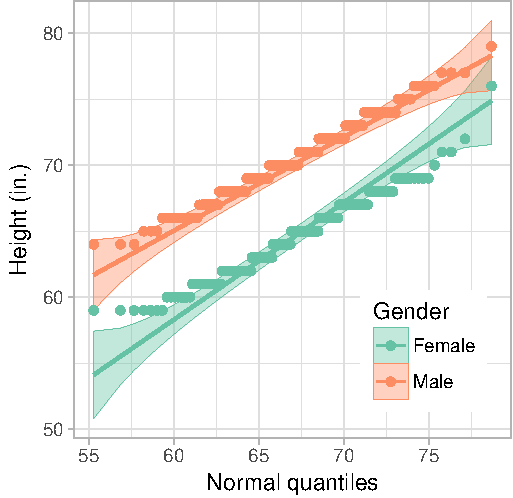
\includegraphics[width=0.4\linewidth]{loy-figures/heights-1} 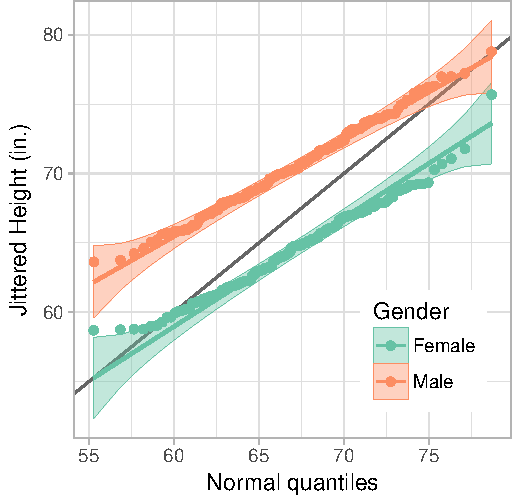
\includegraphics[width=0.4\linewidth]{loy-figures/heights-2} 

}

\caption[Q-Q plots comparing the raw (left) and jittered (right) heights to a normal distribution for a sample of 200 men and 200 women]{Q-Q plots comparing the raw (left) and jittered (right) heights to a normal distribution for a sample of 200 men and 200 women. The distribution on the left is dominated by the discreteness of the data. On the right, using a normal distribution to model people's height is not completely absurd, except for a few extreme outliers.}\label{fig:heights}
\end{figure}
\end{Schunk}

Notice that the same theoretical normal distribution was fit to both
genders as specified in \texttt{dparams}. If we had used the default,
then the MLEs for each gender would be used. As a result, we would be
comparing the two genders over a different range of theoretical
quantiles. By explicity providing parameter estimates for the mean and
standard deviation via \texttt{dparams}, we force the Q-Q plots to use
the same \(x\)-coordinates (theoretical quantiles), which is more useful
when comparing the distribution of these groups.

As seen in Figure \ref{fig:heights}, by using jittering we diminish the
effect that discreteness has on the distribution and brings the observed
distribution much closer to a normal distribution. Unsurprisingly, the
resulting distributions have different means (women are, on average, 6
inches shorter than men in this dataset). Interestingly, the slope of
the two genders is similar, indicating that the same scale parameter
fits both genders' distributions (the standard deviation of height in
the data set is 2.97 inch for men and 2.91 inch for women, see Table
\ref{tab:heights}). The dark line between the two groups in the right
panel of Figure \ref{fig:heights} is the identity line, representing the
theoretical distribution each group is compared to. While the mean is
about half way between the gender means, the standard deviation of the
height based on the whole population is larger, as seen by the steeper
slope of the identity compared to the lines for each group.

\begin{table}

\caption{\label{tab:heights-table}Summary of Iowa residents' heights and weights with corresponding standard deviations by gender and for the total population.\label{tab:heights}}
\centering
\begin{tabular}[t]{lrrrr}
\toprule
SEX & mean height (in) & sd (in) & mean log weight (kg) & sd (kg)\\
\midrule
Male & 70.55 & 2.97 & 9.10 & 0.20\\
Female & 64.51 & 2.91 & 8.89 & 0.23\\
Total & 66.99 & 4.18 & 8.98 & 0.24\\
\bottomrule
\end{tabular}
\end{table}

Unlike respondents' heights, their weights do not seem to be normally
distributed. Figure \ref{fig:weights} shows two Q-Q plots of these data.
The Q-Q plot on the left compares raw weights to a normal distribution.
We see that tails of the observed distribution are heavier than expected
under a normal distribution. On the right, weights are log-transformed.
We see that using a normal distribution for each gender appears to be
reasonable, with the exception of a few extreme outliers. The code used
to create Figure \ref{fig:weights} is shown below:

\begin{Schunk}
\begin{Sinput}
params <- iowa %>% 
  filter(!is.na(WTKG3)) %>% 
  summarize(
    m = mean(WTKG3/100),
    s = sd(WTKG3/100)
  )

sample_ia %>% 
  ggplot(aes(sample = WTKG3 / 100, colour = Gender, fill = Gender)) + 
  stat_qq_band(alpha = 0.4,
               dparams = list(mean = params$m, sd = params$s)) + 
  stat_qq_line(dparams = list(mean = params$m, sd = params$s)) + 
  stat_qq_point(dparams = list(mean = params$m, sd = params$s)) +
  customization +
  ylab("Weight (kg.)")

sample_ia %>% 
  ggplot(aes(sample = log(WTKG3/100), colour=Gender, fill=Gender)) + 
  stat_qq_band(alpha = 0.4,dparams = list(mean = params$m, sd = params$s)) + 
  stat_qq_line(dparams = list(mean = params$m, sd = params$s)) + 
  stat_qq_point(dparams = list(mean = params$m, sd = params$s)) +
  customization +
  ylab("log Weight (kg.)")
\end{Sinput}
\begin{figure}

{\centering 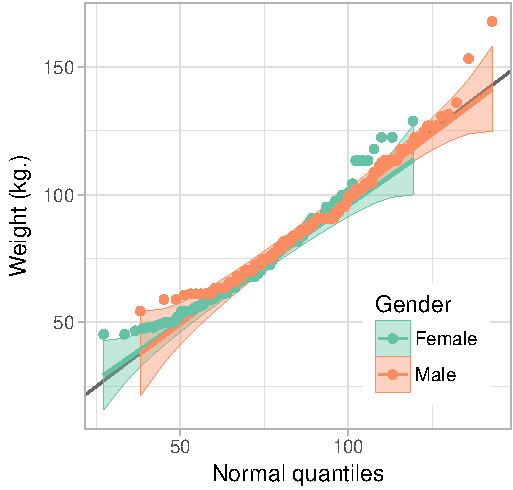
\includegraphics[width=0.4\linewidth]{loy-figures/weights-1} 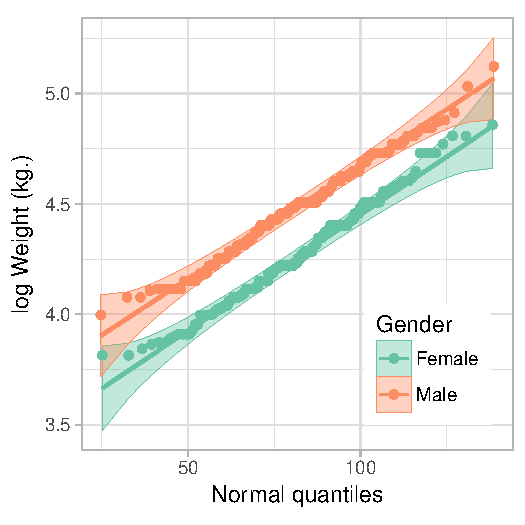
\includegraphics[width=0.4\linewidth]{loy-figures/weights-2} 

}

\caption[Q-Q plots comparing weights to a normal distribution for a sample of 200 men and 200 women]{Q-Q plots comparing weights to a normal distribution for a sample of 200 men and 200 women. Unlike people's height, weight seems to be right skewed with some additional outliers in the left tail (left plot). On the right, weight was log-transfomed before its distribution is compared to a theoretical normal.}\label{fig:weights}
\end{figure}
\end{Schunk}

Instead of log-transforming the observed weights, we can change the
theoretical distribution to a lognormal. Figure \ref{fig:weights-log}
shows two lognormal Q-Q plots, one for each gender. Note the MLEs are
used to parameterize the lognormal distribution for each group since
\texttt{dparams} is not specified:

\begin{Schunk}
\begin{Sinput}
sample_ia %>% 
  ggplot(aes(sample = WTKG3 / 100, colour = Gender, fill = Gender)) +
  geom_abline(colour = "grey40") +
  stat_qq_band(distribution = "lnorm", alpha = 0.4) +
  stat_qq_line(distribution = "lnorm") +
  stat_qq_point(distribution = "lnorm") +
  customization +
  facet_grid(. ~ Gender) +
  xlab("Lognormal quantiles") +
  ylab("Weight (kg.)") +
  theme(legend.position = c(0.9, 0.2))
\end{Sinput}
\begin{figure}

{\centering 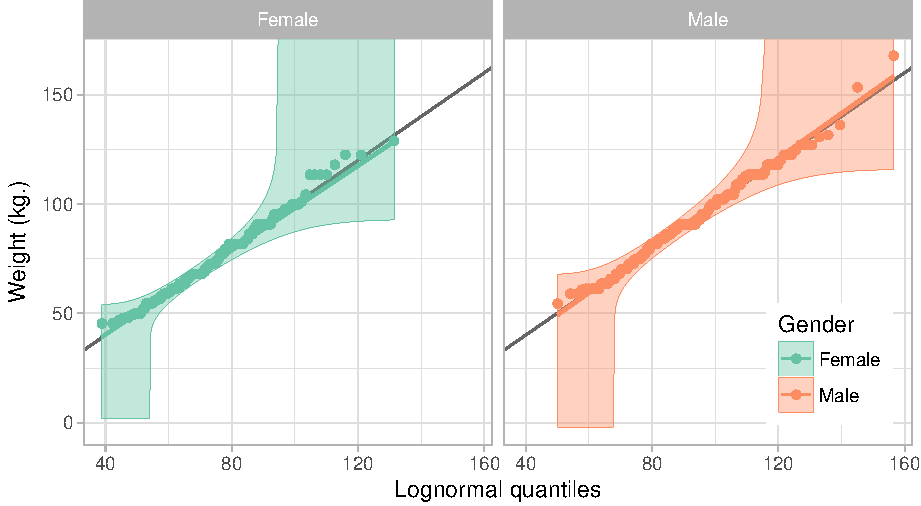
\includegraphics[width=0.9\linewidth]{loy-figures/weights-log-1} 

}

\caption[Q-Q plots comparing weights to a lognormal distribution for a sample of 200 men and 200 women]{Q-Q plots comparing weights to a lognormal distribution for a sample of 200 men and 200 women. The parameters are estimated separately for each gender to specify the lognormal reference distribution for each gender.}\label{fig:weights-log}
\end{figure}
\end{Schunk}

\subsection{Discussion}\label{discussion}

This paper presented the \pkg{qqplotr} package, an extension of
\pkg{ggplot2} that implements Q-Q plots in both the standard and
detrended orientations, along with reference lines and confidence bands.
The examples illustrated how to create Q-Q plots for non-standard
distributions found outside of the \pkg{stats} package, how to create
detrended Q-Q plots, and how to create Q-Q plots when data are grouped.
Further, in the BRFSS example, we illustrated how jittering can be used
in Q-Q plots to better compare discretized data to a continuous
distribution.

While \pkg{qqplotr} provides a complete implementation of Q-Q plot,
there is room for development in future versions. For example, Q-Q plots
are members of the larger probability plotting family, so future
versions of \pkg{qqplotr} will likely include additional members of that
family.

Finally, we have made design choices in \pkg{qqplotr} that we believe
are in line with best practices for distributional assessment, but the
implementation is flexible enough to allow for easy customization. For
example, maximum likelihood is used to estimate the parameters of the
proposed model, but if outliers are present robust estimators may be
desirable, such as if you are comparing the empirical distribution to a
normal distribution. In this scenario, robust estimates of the location
and scale can be obtained using the \pkg{robustbase} package
\citep{robustbase}, and specified using the \texttt{dparams} parameter
directly. This is especially useful if you wish to use the parametric
bootstrap to build confidence bands. Similarly, \texttt{stat\_qq\_line}
implements two types of reference lines: the identity line, and the
traditional Q-Q line that passes through two quantiles of the
distributions, such as the first and third quartiles. While those are
the most conventionally used reference lines, alternative ones can be
quickly implemented using \texttt{ggplot2::geom\_abline} by specifying
the slope and intercept. By default, the Q-Q line is used; however, this
is not always the most appropriate choice. In order to \emph{test}
whether the data follow a specific distribution, the reference line
should be used rather than using the data twice: once to estimate the
parameters, and once for comparison.

\bibliography{loy}

\subsection{Acknowledgements}\label{acknowledgements}

This work was partially funded by Google Summer of Code 2017.

\section{Changes}\label{changes}

\begin{itemize}
\tightlist
\item
  added Davison reference for point-wise confidence intervals
\end{itemize}

\address{%
Alexandre Almeida\\
University of Campinas\\
Institute of Computing\\ Campinas, Brazil 13083-852\\
}
\href{mailto:almeida.xan@gmail.com}{\nolinkurl{almeida.xan@gmail.com}}

\address{%
Adam Loy\\
Carleton College\\
Department of Mathematics and Statistics\\ Northfield, MN 55057\\
}
\href{mailto:aloy@carleton.edu}{\nolinkurl{aloy@carleton.edu}}

\address{%
Heike Hofmann\\
Iowa State University\\
Department of Statistics\\ Ames, IA 50011-1210\\
}
\href{mailto:hofmann@iastate.edu}{\nolinkurl{hofmann@iastate.edu}}

